\section{Intel Cyclone V SE device}\label{sec:intel}

Similarly to the assessment of the ZYNQ-7010 device, the same three systems depicted in Figure~\ref{fig:evaluation_circuit} were implemented and targeted in the Cyclone V SE device. Since the Cyclone V device family only has one on-chip high-performance port that connects the \ac{FPGA} to the DDR controller through the \ac{HPS}, a single \ac{DMA} engine was used in each system. The used \ac{DMA} engine was Intel's \ac{MSGDMA}, which revealed capable of fully-exploiting the bandwidth of the \ac{F2S} interface. The Intel's \ac{MSGDMA} allows three configurations regarding its input and output interfaces: AXI3-to-AXI3, AXI3-to-Avalon-Stream, and Avalon-Stream-to-AXI3. Furthermore, the \ac{MSGDMA} also includes an internal data \ac{FIFO}, which allows simplifying the system to assess the duplex bandwidth by using the \ac{MSGDMA} in the configuration AXI3-to-AXI3 and connecting both interfaces to the \ac{F2S} port directly, as shown in Figure~\ref{fig:intel_duplex}. Note that both the AXI3 interfaces of the \ac{MSGDMA} can be connected to the \ac{F2S} port even if they have \SI{256}{\bit} each. This is only possible because each of these interfaces is single-sided (one interface only reads and the other only writes), and the \ac{F2S} port is full-duplex. For testing the \ac{HPS}-to-\ac{FPGA} and the \ac{FPGA}-to-\ac{HPS} bandwidths, the \ac{MSGDMA} was configured as AXI3-to-Avalon-Stream and Avalon-Stream-to-AXI3, respectively. Additionally, two simple circuits were developed to absorb the stream generated by the \ac{MSGDMA} in the configuration AXI3-to-Avalon-Stream and generate a data stream to be absorbed by the \ac{MSGDMA} in the configuration Avalon-Stream-to-AXI3. In resemblance to the system targeting the Xilinx device, the circuit to absorb the stream consists of a single wire connected to the \textit{ready} signal of the Avalon-Stream master interface. On the other hand, the circuit to produce a data stream to be transmitted to the \ac{MSGDMA} engine is simpler than its Xilinx counterpart. The streaming protocol used by the Xilinx \ac{DMA} device is the AXI4-Stream protocol, which features signal indicating the end of the stream. Therefore, a \ac{FSM} is needed to count the elements of the stream and activate the \textit{last} signal during the transmission of the stream's last element. However, the streaming protocol used by Intel's \ac{MSGDMA} (Avalon-Stream~\cite{intel2020avalon}) does not have a signal indicating the end of the stream. Thus, there is no need for a \ac{FSM}. To produce a constant stream, it only takes to set the \textit{data} bus to a constant and the \textit{valid} signal to high. Figures~\ref{fig:intel_h2f} and \ref{fig:intel_f2h} illustrate the systems to evaluate the \ac{HPS}-to-\ac{FPGA} and \ac{FPGA}-to-\ac{HPS} bandwidths, respectively.

\begin{figure}[!b]
    \centering
    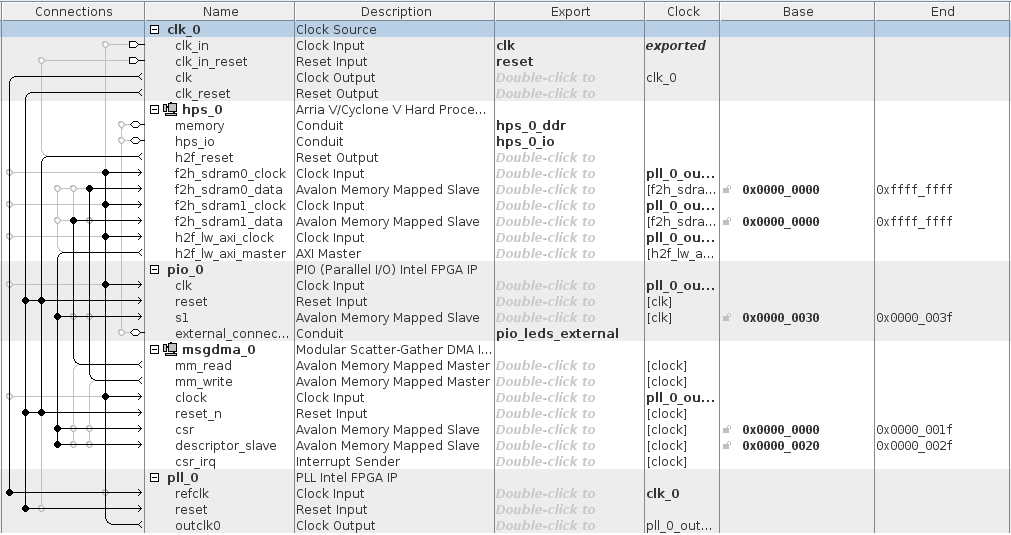
\includegraphics[width=\linewidth]{figures/intel_duplex.png}
    \caption{Schematic of the system to assess the duplex bandwidth of the on-chip high-performance interfaces of the Intel device, as shown in the Platform Designer tool of Intel Quartus Prime.}
    \label{fig:intel_duplex}
\end{figure}

\begin{figure}[!t]
    \centering
    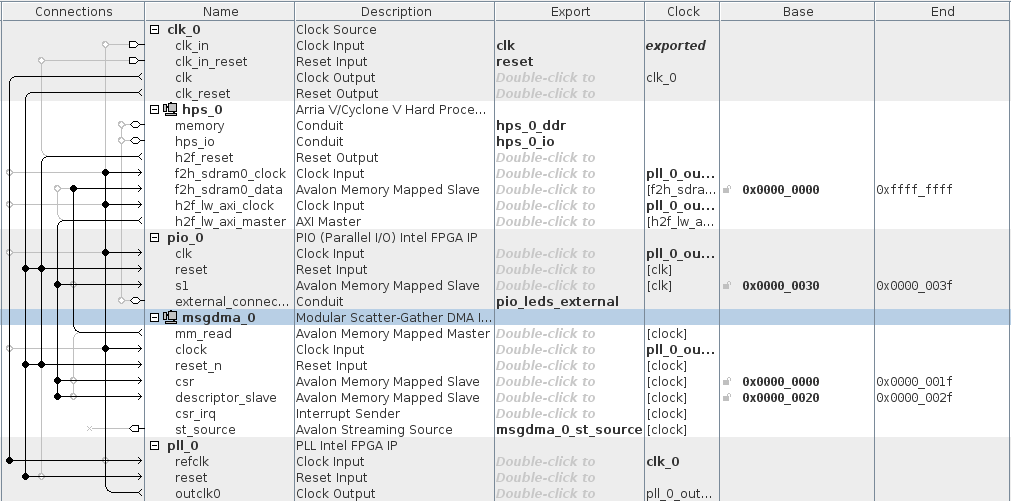
\includegraphics[width=\linewidth]{figures/intel_h2f.png}
    \caption{Schematic of the system to assess the \ac{HPS}-to-\ac{FPGA} bandwidth of the on-chip high-performance interfaces of the Intel device, as shown in the Platform Designer tool of Intel Quartus Prime.}
    \label{fig:intel_h2f}
\end{figure}

\begin{figure}[!t]
    \centering
    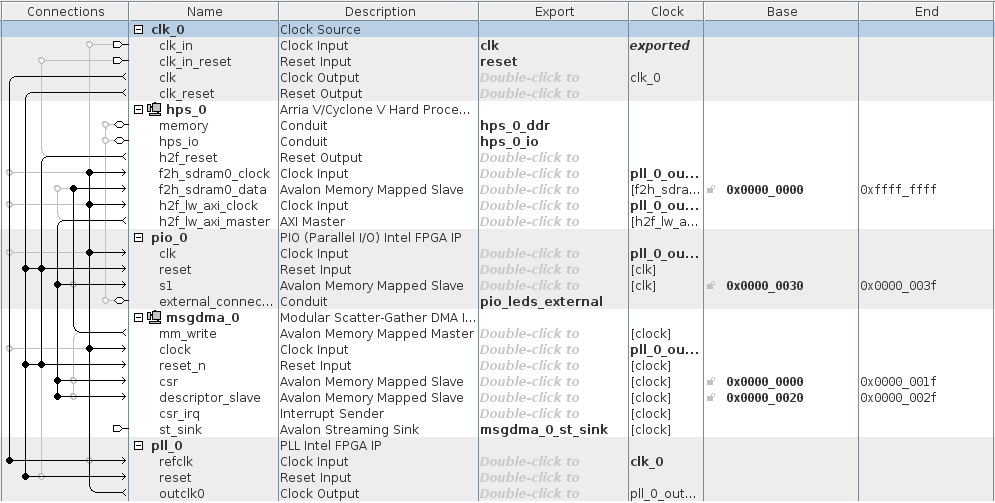
\includegraphics[width=\linewidth]{figures/intel_f2h.png}
    \caption{Schematic of the system to assess the \ac{FPGA}-to-\ac{HPS} bandwidth of the on-chip high-performance interfaces of the Intel device, as shown in the Platform Designer tool of Intel Quartus Prime.}
    \label{fig:intel_f2h}
\end{figure}

In contrast with the software framework for controlling and monitoring the \ac{FPGA}-implemented circuits in the Xilinx device (which was bare-metal), the software used to control the \ac{FPGA} components on the Intel device was developed to be executed in Linux environment. This implementation choice had to do with the poorer bare-metal development support provided by Intel tools when comparing to Xilinx's more powerful and automated tools. For instance, compiling a bare-metal application for Intel devices requires the developer to write a linker script by hand (there is no tool to generate the linker script automatically). Although Intel provides linker scripts that can be used out-of-the-box, they only work for certain applications. Another possibility is to use the ARM compiler, instead of the default Intel bare-metal compiler, which requires the user to write a scatter file. Although scatter files are usually much less verbose than linker scripts, their syntax is also complex. Naturally, the examples of scatter files provided by ARM also have a limited scope. In contrast with bare-metal, Linux development is much more powerful and there are simple known techniques to overcome issues such as addressing memory-mapped peripherals through their physical addresses, or reserve part of the DDR memory to be used directly by \ac{DMA} engines without needing to translate virtual addresses. As explained by Kashani \textit{et al.}~\cite{sahandSoCTutorial}, the physical addresses of the memory-mapped peripherals can be accessed from the Linux system using the function \texttt{mmap} to map those addresses into addresses in the application addressing space. To reserve part of the DDR to be used directly by \ac{DMA} engines, it is possible to assign only a sub-region of the DDR to the Linux kernel at boot time, leaving the upper addresses free. By default, the upper part of the DDR that is not used by the Linux kernel is ignored by the operating system and is initialized as non-cacheable memory. However, it can still be accessed using the same method to address the memory-mapped peripherals, using the \texttt{mmap} function to map the physical addresses of the upper DDR region into addresses in the application addressing space.

\subsection{Experimental Results}

The three systems to evaluate the bandwidth of the on-chip high-performance interfaces of the Cyclone V device were implemented using Intel Quartus Prime 18.1 with a \ac{FPGA} operation frequency of \SI{100}{\mega\hertz}. The \ac{MSGDMA} was configured for a maximum burst size of sixteen, and a maximum stream size of \SI{256}{\mega\byte}. The \ac{F2S} port was tested for 32, 64, 128 and 256-bit configurations. The hardware requirements of the implemented systems are listed in Table~\ref{tab:hardware_intel}, in Appendix~\ref{sec:hardware_resources}.

Table \ref{tab:intel_results_regular} summarizes the performance results obtained using all the three systems. The rows painted in yellow correspond to sub-optimal configurations whose bandwidth is degraded compared with the theoretically expected. The highest bandwidth (\SI{2779.05}{\mega\byte\per\second}) was achieved for \ac{HPS}-to-\ac{FPGA} transfers using all the \SI{256}{bit} of the \ac{F2S} port, which is compatible with the results obtained by G{\"{o}}bel \textit{et al.}. Similarly to the Xilinx device, for configurations where the \ac{F2S} interface is wider, the bandwidth is degraded. Furthermore, that effect is exaggerated by the lower operating frequency of the DRAM connected to the Cyclone V device comparing with the one connected to the ZYNQ-7000 device, which leads to a lower DRAM bandwidth. It is also worth noticing that the maximum bandwidth allowed for duplex transfers is lower than the one associated with single-sided transfers. This effect is also visible in the results regarding the Xilinx device and can be attributed to the entropy generated at the DRAM controller level when multiplexing the DDR ports to read and write data at data rates close to the DRAM's limit. This hypothesis is supported by the higher standard deviations associated with the results of experiments using those configurations, which indicate that they are not completely deterministic.

\begin{table}[!b]
\centering
\caption{Expected and observed bandwidth and respective system efficiency for several system configurations using \ac{F2S} ports of the Cyclone V device. Each configuration was tested 200 times for \SI{32}{\mebi\byte} data blocks. The \ac{FPGA} operating frequency was \SI{100}{\mega\hertz}. Note that H2F stands for \ac{HPS}-to-\ac{FPGA}, and F2H means \ac{FPGA}-to-\ac{HPS}.}
\label{tab:intel_results_regular}
\begin{tabular}{l|c|r|r|r|r|r|r|}
\cline{2-8}
                                                                        &                                                                                                & \multicolumn{5}{c|}{\textbf{Bandwidth [\si{\mega\byte\per\second}]}}                                                                                                                                                      & \multicolumn{1}{c|}{}                                           \\ \cline{3-7}
                                                                        &                                                                                                & \multicolumn{1}{c|}{}                                    & \multicolumn{4}{c|}{\textbf{Observed}}                                                                                                                         & \multicolumn{1}{c|}{}                                           \\ \cline{4-7}
                                                                        & \multirow{-3}{*}{\textbf{\begin{tabular}[c]{@{}c@{}}Channel\\ Width [\si{\bit}]\end{tabular}}} & \multicolumn{1}{c|}{\multirow{-2}{*}{\textbf{Expected}}} & \multicolumn{1}{c|}{\textbf{Average}} & \multicolumn{1}{c|}{\textbf{Minimum}} & \multicolumn{1}{c|}{\textbf{Maximum}} & \multicolumn{1}{c|}{$\mathbf{\sigma}$} & \multicolumn{1}{c|}{\multirow{-3}{*}{\textbf{Efficiency [\%]}}} \\ \hline
\multicolumn{1}{|l|}{}                                                  & \textbf{32}                                                                                    & 800.00                                                   & 799.59                                & 799.04                                & 799.91                                & 0.1279                                 & 99.95                                                           \\ \cline{2-8} 
\multicolumn{1}{|l|}{}                                                  & \textbf{64}                                                                                    & 1600.00                                                  & 1579.80                               & 1563.76                               & 1583.54                               & 3.1448                                 & 98.74                                                           \\ \cline{2-8} 
\multicolumn{1}{|l|}{}                                                  & \cellcolor[HTML]{FFFF00}\textbf{128}                                                           & \cellcolor[HTML]{FFFF00}3200.00                          & \cellcolor[HTML]{FFFF00}2019.26       & \cellcolor[HTML]{FFFF00}1836.18       & \cellcolor[HTML]{FFFF00}2023.30       & \cellcolor[HTML]{FFFF00}13.9767        & \cellcolor[HTML]{FFFF00}63.10                                   \\ \cline{2-8} 
\multicolumn{1}{|l|}{\multirow{-4}{*}{\textbf{\rotatebox{90}{Duplex}}}} & \cellcolor[HTML]{FFFF00}\textbf{256}                                                           & \cellcolor[HTML]{FFFF00}3200.00                          & \cellcolor[HTML]{FFFF00}2037.16       & \cellcolor[HTML]{FFFF00}1885.93       & \cellcolor[HTML]{FFFF00}2039.91       & \cellcolor[HTML]{FFFF00}13.1620        & \cellcolor[HTML]{FFFF00}63.66                                   \\ \hline
\multicolumn{1}{|l|}{}                                                  & \textbf{32}                                                                                    & 400.00                                                   & 399.81                                & 399.69                                & 399.96                                & 0.0299                                 & 99.95                                                           \\ \cline{2-8} 
\multicolumn{1}{|l|}{}                                                  & \textbf{64}                                                                                    & 800.00                                                   & 799.60                                & 797.81                                & 799.87                                & 0.1862                                 & 99.95                                                           \\ \cline{2-8} 
\multicolumn{1}{|l|}{}                                                  & \textbf{128}                                                                                   & 1600.00                                                  & 1569.88                               & 1561.47                               & 1570.90                               & 1.5062                                 & 98.12                                                           \\ \cline{2-8} 
\multicolumn{1}{|l|}{\multirow{-4}{*}{\textbf{\rotatebox{90}{H2F}}}}    & \cellcolor[HTML]{FFFF00}\textbf{256}                                                           & \cellcolor[HTML]{FFFF00}3200.00                          & \cellcolor[HTML]{FFFF00}2779.05       & \cellcolor[HTML]{FFFF00}2736.46       & \cellcolor[HTML]{FFFF00}2790.85       & \cellcolor[HTML]{FFFF00}5.9443         & \cellcolor[HTML]{FFFF00}86.85                                   \\ \hline
\multicolumn{1}{|l|}{}                                                  & \textbf{32}                                                                                    & 400.00                                                   & 399.81                                & 399.70                                & 399.95                                & 0.0333                                 & 99.95                                                           \\ \cline{2-8} 
\multicolumn{1}{|l|}{}                                                  & \textbf{64}                                                                                    & 800.00                                                   & 799.59                                & 797.83                                & 799.87                                & 0.2206                                 & 99.95                                                           \\ \cline{2-8} 
\multicolumn{1}{|l|}{}                                                  & \textbf{128}                                                                                   & 1600.00                                                  & 1576.78                               & 1574.66                               & 1579.18                               & 1.8717                                 & 98.55                                                           \\ \cline{2-8} 
\multicolumn{1}{|l|}{\multirow{-4}{*}{\textbf{\rotatebox{90}{F2H}}}}    & \cellcolor[HTML]{FFFF00}\textbf{256}                                                           & \cellcolor[HTML]{FFFF00}3200.00                          & \cellcolor[HTML]{FFFF00}2464.66       & \cellcolor[HTML]{FFFF00}2137.91       & \cellcolor[HTML]{FFFF00}2473.06       & \cellcolor[HTML]{FFFF00}32.3298        & \cellcolor[HTML]{FFFF00}77.02                                   \\ \hline
\end{tabular}
\end{table} %

Concluding the analysis of the Cyclone V device family, a final scenario based on the system to evaluate the duplex bandwidth was considered. The \ac{F2S} port was configured to use only \SI{64}{bit} and the system was implemented targeting an operation frequency of \SI{100}{\mega\hertz}. This experiment consisted of transferring streams of multiple sizes from the \ac{HPS} to the \ac{FPGA} and back to the \ac{HPS}. Each stream size was tested 200 times, and the results were averaged. Figure \ref{fig:intel_results_var_size} illustrates the results of this experiment. Results show that small stream sizes only achieve a fraction of the theoretical maximum bandwidth allowed by the \ac{F2S} port. Only for stream sizes bigger than \SI{512}{\kibi\byte} a real bandwidth of more than 90\% of the theoretical maximum is achieved.

\begin{figure}[t]
    \centering
    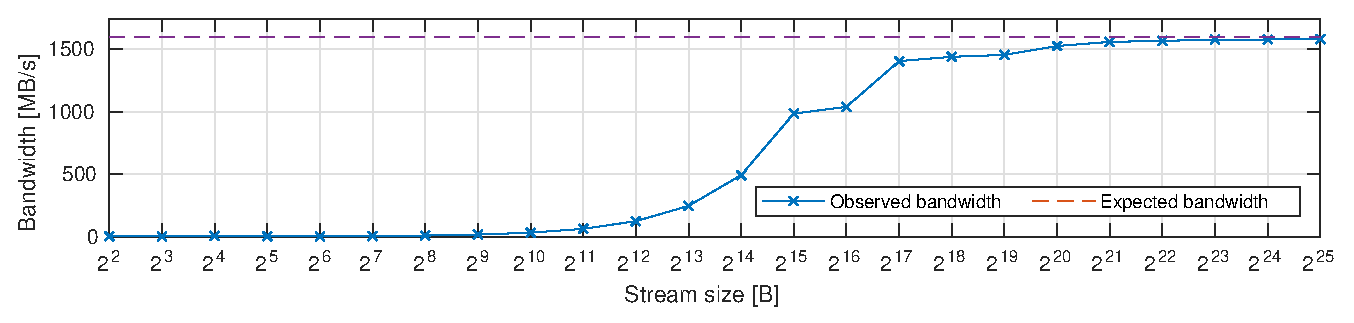
\includegraphics[width=\linewidth]{figures/intel_var_stream_size.eps}
    \caption{Observed duplex bandwidth for different stream sizes. The system was designed using a 64-bit \ac{F2S} port and a loop-back \ac{FIFO}, allowing to fully exploit the duplex bandwidth of the \ac{F2S} port. The \ac{FPGA} operation frequency is \SI{100}{\mega\hertz}. Each data point represents the average of 200 transactions of the same size. The maximum standard deviation was \SI{42.19}{\mega\byte\per\second}.}
    \label{fig:intel_results_var_size}
\end{figure}